\subsection{Descrizione dell'esperimento}
L'esperimento è stato eseguito utilizzando un circuito logico preconfigurato, in cui la cablatura e l'ottimizzazione del punto di lavoro sono stati già completati. Il principio operativo dell'esperimento si basa sulla coincidenza dei segnali di tre rivelatori disposti in cascata. Come illustrato nella figura di riferimento\footnote{Handouts$\_$LMN$\_$2024$\_$V$4.1$$\_$muon.pdf del Professore S. D'Auria}, il setup sperimentale prevede un primo rivelatore, sopra il quale è possibile posizionare un assorbitore in piombo per eliminare i muoni meno energetici e una parte dei muoni negativi. Successivamente, troviamo un secondo rivelatore, un attenuatore in ottone e infine un terzo rivelatore.
 %IMMAGINE Apparato muone
\begin{figure}[htp!]
  \centering
  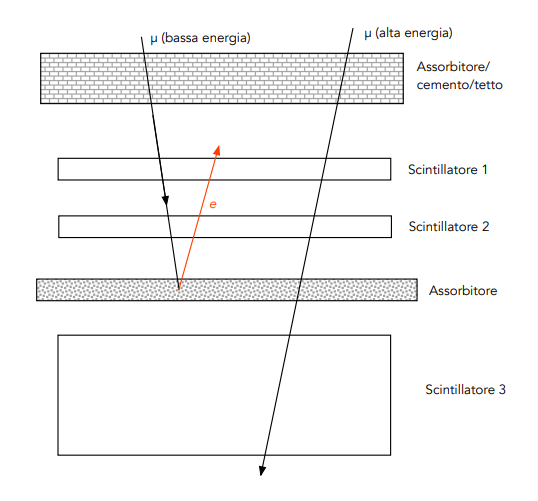
\includegraphics[scale=0.6]{Materiali e Strumentazioni/Apparato muone.png} 
  \caption{Schema semplificato dell'apparato sperimentale}
\end{figure}
Nel nostro esperimento, selezioniamo muoni con sufficiente energia per attraversare i due strati di cemento e, possibilmente, anche l'assorbitore in piombo. Mentre i muoni troppo poco energetici si fermano prima, i muoni troppo energetici non verranno contati in quanto rivelati nel terzo scintillatore. Una volta che i muoni vengono fermati, perdono il loro boost relativistico e decadono secondo il loro tempo proprio, come descritto nella sezione teorica. Ad esempio, l decadimento dei muoni positivi, produce positroni che vengono emessi preferenzialmente verso l'alto.

Un aspetto cruciale del setup sperimentale è la coincidenza temporale dei segnali tra gli scintillatori. Per selezionare i muoni che si fermano nell'assorbitore, richiediamo che ci sia un segnale contemporaneo nel primo e nel secondo scintillatore, ma non nel terzo. Questo costituisce il nostro segnale per avviare il "cronometro". Per misurare tempi dell'ordine dei microsecondi, è fondamentale che gli scintillatori siano rapidi, ovvero che producano un segnale luminoso molto più veloce rispetto al tempo che intendiamo misurare. Per tale scopo, vengono utilizzati scintillatori plastici, i cui dettagli saranno discussi nella sezione dedicata.

Quando un muone si ferma nell'attenuatore in ottone, decade emettendo un elettrone con energia variabile da $0$ a $50,\text{MeV}$. La parte alta dello spettro energetico è sufficiente per permettere all'elettrone di uscire dall'assorbitore e attraversare i due scintillatori plastici superiori. Per fermare il cronometro, utilizziamo lo stesso segnale di coincidenza dei due scintillatori (S1 e S2, ma non S3), entro una finestra temporale specifica di alcuni microsecondi dal primo segnale.
\subsection{Rivelatori e Circuito}
I rivelatori utilizzati all'interno di questo esperimento sono composti da tre scintillatori plastici organici accoppiati a dei fotomoltiplicatori. La scelta di utilizzare questo tipo di scintillatori risiede nella necessità di avere una risoluzione temporale compatibile rispetto alla quantità che si vuole misurare. Per quanto riguarda questo aspetto i rivelatori organici sono preferibili ai rivelatori inorganici in cui invece è migliore la Light Yield.

Il circuito, visibile nella fig. \ref{figura:circuito} è costituito da una coincidence unit che in elettronica è anche riconosciuta come una porta AND. Nel nostro caso la usiamo sia come segnale di "start" che come segnale di "stop". L'uscita ha un valore logico 1 se abbiamo che S1, S2 e l'entrata negata di S3 danno tutti come valore 1. Questo corrisponde alla situazione descritta in precedenza in cui il muone passa per i primi due scintillatori ma non nel terzo, fermandosi nell'attenuatore. Il segnale viene mandato in una entrata della TTL e nella time unit che genera un segnale di durata fissa controllata da un impulso di start e un impulso di stop. Un'altra uscita è l'end marker che termina il segnale dopo un tempo che è possibile impostare tramite delle manopole. Dalla Time Unit ci sono due uscite: la prima è collegata con l'ingresso veto di start per non far partire una ulteriore misura durante il periodo del segnale della time unit. La seconda viene ritardata ed entra nella coincidence unit in cui il segnale sarà dato se e solo se la misura ha avuto uno start (Ch4) e viene rivelato l'elettrone o il positrone dal S1 S2 ma non dal S3. Questo genera un segnale che finisce nella FAN-In/FAN-Out (in elettronica anche definito come OR). Quest'ultimo ha come seconda entrata l'end marker della time unit. Quindi il FAN-In/FAN-Out fornisce un segnale logico 1 se riceve il segnale di stop (passa l'elettrone o il positrone e quindi avviene la misura) oppure quando riceve il segnale del end-marker. Il segnale viene raccolto nella seconda entrata del TTL e successivamente i due segnali della TTL di start e stop entrano nella TDC responsabile di misurare il tempo tra i due segnali.
 %IMMAGINE coso
\begin{figure}[htp!]
  \centering
  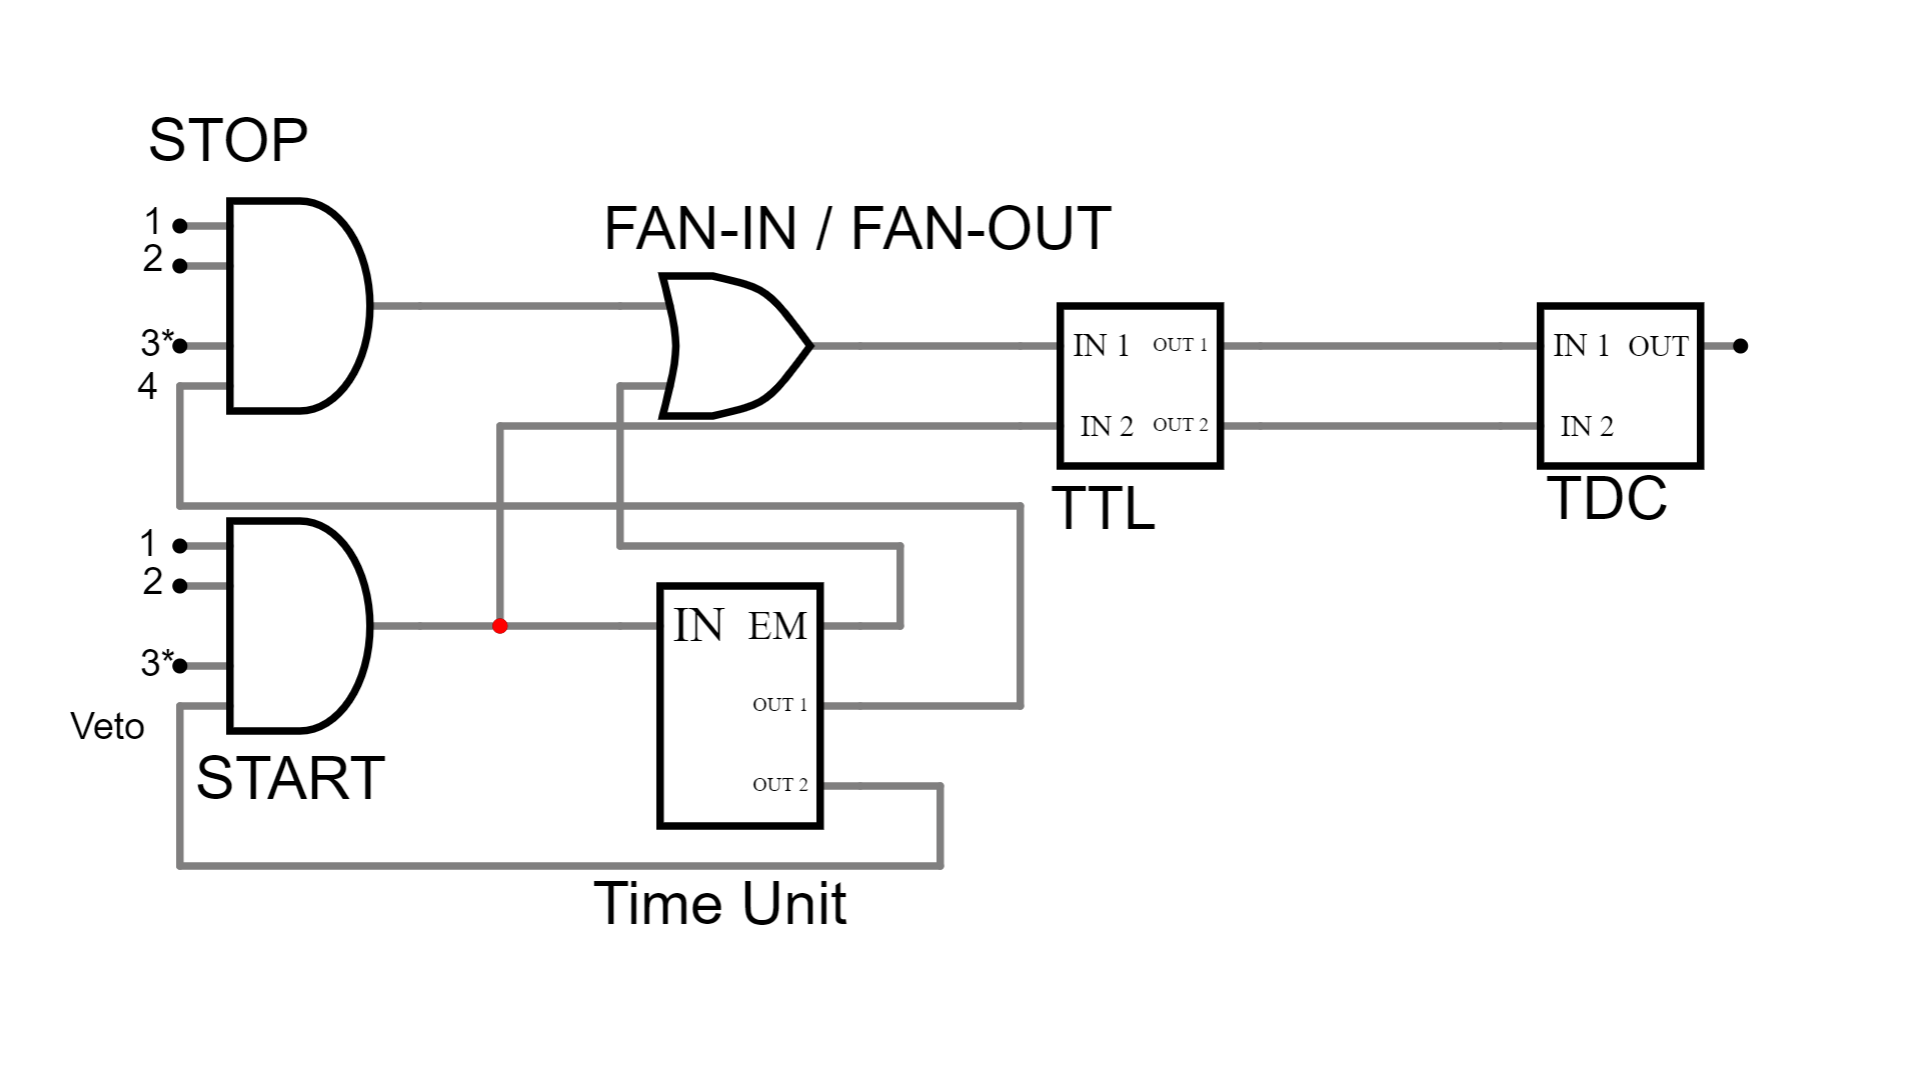
\includegraphics[scale=0.35]{Materiali e Strumentazioni/coso2.png} 
  \caption{In questa immagine è possibile visualizzare lo schema logico del circuito descritto.}
  \label{figura:circuito}
\end{figure}
